\newpage
\section{Methodology}\label{ch:method}
\subsection{Problem Definition}
For each row dated $t$ the task is three-class classification of the next trading day's return $r_{t\to t+1}$ into $y_t\in\{\text{Fall},\text{Neutral},\text{Rise}\}$. The inputs available are a window $X_t\in\mathbb{R}^{10\times12}$ of price features ending at $t$, a news representation $n_t$ built from the headlines dated $t$, and a regime label $g_t\in\{\text{Low-vol},\text{Mid-vol},\text{High-vol}\}$. The primary metric is Macro-F1,
\[
\mathrm{Macro\text{-}}\Fone=\frac13\sum_{c\in\{\text{Fall},\text{Neutral},\text{Rise}\}}\Fone^{(c)},\qquad
\Fone^{(c)}=\frac{2\,P_cR_c}{P_c+R_c},
\]
with accuracy and balanced accuracy (mean per-class recall) reported alongside.

\subsection{Price Features}
Raw price levels drift from about 100 to 340 over the sample, so test-period inputs would sit far outside the training range. Twelve \emph{scale-free} features are therefore computed from the recovered daily series (Table~\ref{tab:features}).
\begin{table}[H]
\centering
\begin{tabular}{ll}
\toprule
Name & Definition\\
\midrule
\texttt{ret} & daily close-to-close return\\
\texttt{oc} & close/open $-1$\\
\texttt{hl} & (high $-$ low)/close\\
\texttt{lvol\_rel} & log volume minus its trailing 20-day mean\\
\texttt{macd\_n} & MACD/close\\
\texttt{rsi}, \texttt{cci}, \texttt{dx} & 30-day RSI, CCI and DX, each divided by 100\\
\texttt{bollpos} & (close $-$ lower band)/(upper $-$ lower band)\\
\texttt{bollw} & (upper $-$ lower band)/close\\
\texttt{c\_sma30}, \texttt{c\_sma60} & close/30-day (60-day) simple moving average $-1$\\
\bottomrule
\end{tabular}
\caption{The 12 scale-free price features. Indicator columns (MACD, RSI, CCI, DX, Bollinger bands, moving averages) are those supplied by the dataset.}\label{tab:features}
\end{table}
Features are standardised with a mean and standard deviation estimated on the rows allowed by the protocol (Section~\ref{sec:protocols}) and clipped to $\pm5$ standard deviations to limit the effect of extreme 2020 values.

\subsection{News Representation}
Headlines of day $t$ are encoded by the frozen \texttt{ProsusAI/finbert} model \cite{araci2019} (maximum 64 tokens per headline, batch size 256). Up to 50 headlines per day are sampled with a fixed seed. Two representations are produced per day:
\begin{enumerate}
\item the \textbf{embedding}: the mean of the 768-dimensional headline representations; and
\item the \textbf{sentiment}: the mean of the three FinBERT class probabilities (positive, negative, neutral).
\end{enumerate}
FinBERT is never fine-tuned; all learning on the news side happens in a small downstream layer.

\subsection{Market Regimes}
Two regime features use only prices up to the row's date: the 20-day return $\mathrm{ret}_{20}=C_t/C_{t-20}-1$ and the log of the 20-day standard deviation of daily returns, $\log\sigma_{20}$. The logarithm is used because volatility is right-skewed, so that clusters are not dominated by a few crashes. After standardisation, \textbf{$k$-means with $k=3$} (ten initialisations, fixed seed) assigns each day to a cluster. Clusters are named \emph{Low-vol}, \emph{Mid-vol} and \emph{High-vol} purely by ranking their mean log-volatility; no economic meaning beyond that ranking is assumed.

For the strict protocol the scaler and clustering are fitted on training rows only; for the looser protocols they are fitted on all rows. The two assignments agree on 93.6\% of rows (92.3\% in train, 98.1\% in validation, 94.9\% in test).

\begin{table}[H]
\centering
\begin{tabular}{lrrrrr}
\toprule
Regime & $n$ (train) & mean $\mathrm{ret}_{20}$ & mean $\sigma_{20}$ & mean next-day ret. & share\\
\midrule
Low-vol & 700 & 0.0185 & 0.0055 & $-0.0000$ & 0.479\\
Mid-vol & 411 & 0.0319 & 0.0103 & 0.0009 & 0.281\\
High-vol & 351 & $-0.0363$ & 0.0126 & 0.0010 & 0.240\\
\bottomrule
\end{tabular}
\caption{Regime statistics on training rows (strict-protocol fit).}\label{tab:regimestats}
\end{table}
Regimes persist (Table~\ref{tab:transition}): the daily probability of staying in Low-vol is 0.961, and the median run length is 15 trading days for Low-vol but only 4 for Mid-vol and High-vol, so the intermediate and high regimes switch frequently. The regime mix also changes across splits: High-vol accounts for 24\% of rows in train, 24\% in validation and 25\% in test, whereas Low-vol falls from 64\% in validation to 39\% in test.
\begin{table}[H]
\centering
\begin{tabular}{lccc}
\toprule
From $\backslash$ To & Low-vol & Mid-vol & High-vol\\
\midrule
Low-vol & 0.961 & 0.017 & 0.021\\
Mid-vol & 0.058 & 0.869 & 0.073\\
High-vol & 0.016 & 0.109 & 0.875\\
\bottomrule
\end{tabular}
\caption{Daily regime transition matrix (strict-protocol model).}\label{tab:transition}
\end{table}
\figpage{regimes_overview.png}{\textwidth}{Left: SPY close coloured by regime (strict fit); dashed lines mark the validation and test starts. Right: training rows in regime-feature space with the three cluster centres.}

Across all rows, the label mix differs strongly by regime: the share of Neutral next days is 64.2\% in Low-vol, 54.9\% in Mid-vol and only 28.8\% in High-vol, where Rise (40.6\%) and Fall (30.6\%) dominate. Regimes therefore carry information about the \emph{size} of the next move rather than its sign.

\subsection{Model Family}
All learned models share one architecture whose branches are switched on or off (Figure~1 in the abstract; Table~\ref{tab:models}).
\begin{table}[H]
\centering
\begin{tabular}{llp{6.6cm}}
\toprule
Model & Inputs & Purpose\\
\midrule
M0 & training majority class & deterministic baseline\\
M0r & uniform random guess & chance floor for Macro-F1\\
M1 & price window & price-only benchmark\\
M2 & price + FinBERT embedding & multimodal benchmark\\
M3 & price + embedding + regime & regime-aware multimodal model\\
M4 & embedding only & news-only ablation\\
M5 & regime only & regime-only ablation\\
M6 & price + 3 sentiment scores & compact news-fusion model (added post hoc)\\
\bottomrule
\end{tabular}
\caption{Model family.}\label{tab:models}
\end{table}
The branches are: an \textbf{LSTM} \cite{hochreiter1997} with 64 hidden units whose last hidden state (with dropout 0.2) summarises the price window; a \textbf{news branch} that maps the news vector (768 dimensions for the embedding, 3 for the sentiment) through a linear layer to 64 units with ReLU and dropout; and a \textbf{regime branch}, an embedding of the three regime ids into 8 dimensions. Active branch outputs are concatenated and passed to a head of Linear$(\cdot\to64)$, ReLU, dropout, Linear$(64\to3)$ with softmax cross-entropy.

An additional gated variant (M7), in which a regime-conditioned gate $g=\sigma(W[z_{\text{price}};z_{\text{news}};e_{\text{regime}}])$ mixes the price and news embeddings as $z=g\odot z_{\text{price}}+(1-g)\odot z_{\text{news}}$, is implemented in the code repository. M7 was \emph{not} run on the real data and is not part of the reported results; it is left as future work (Chapter~\ref{ch:conclusion}).

\subsection{Training Procedure}
\begin{defbox}
\textbf{Frozen settings (never tuned on the test set).} Adam optimiser, learning rate $10^{-3}$, weight decay $10^{-4}$, batch size 64, at most 50 epochs, early stopping with patience 8 on \emph{validation} Macro-F1, class-weighted cross-entropy (weights inversely proportional to training class counts), input clipping at $\pm5$ standard deviations. LSTM hidden size 64, dropout 0.2, news output 64, regime embedding 8. Ten seeds (0--9).
\end{defbox}
Hyper-parameters were chosen once, before the main experiments, from conventional values and were not searched. The checkpoint with the best validation Macro-F1 is used for the reported test predictions. The random guesser M0r draws labels uniformly at random with the run's seed.

\subsection{Evaluation Protocols}\label{sec:protocols}
The same models are evaluated under three protocols (Figure~\ref{fig:protocols}) that differ in how data are split and which rows are used to fit preprocessing and regimes.
\begin{table}[H]
\centering
\begin{tabular}{llll}
\toprule
Protocol & Split & Scalers fitted on & Regimes fitted on\\
\midrule
P1 & random (same sizes) & all rows & all rows\\
P2 & chronological & all rows & all rows\\
P3 (primary) & chronological & train rows only & train rows only\\
\bottomrule
\end{tabular}
\caption{Evaluation protocols.}
\end{table}
P1 is deliberately invalid and serves as a permissive reference; P3 is the primary benchmark for all scientific conclusions. In P1 a different random split is drawn for each seed with the same train/validation/test sizes, so the P1 test sample differs from the P2/P3 test sample; the gaps between protocols therefore mix leakage and sampling effects (Chapter~\ref{ch:discussion}).
\begin{figure}[H]
\centering
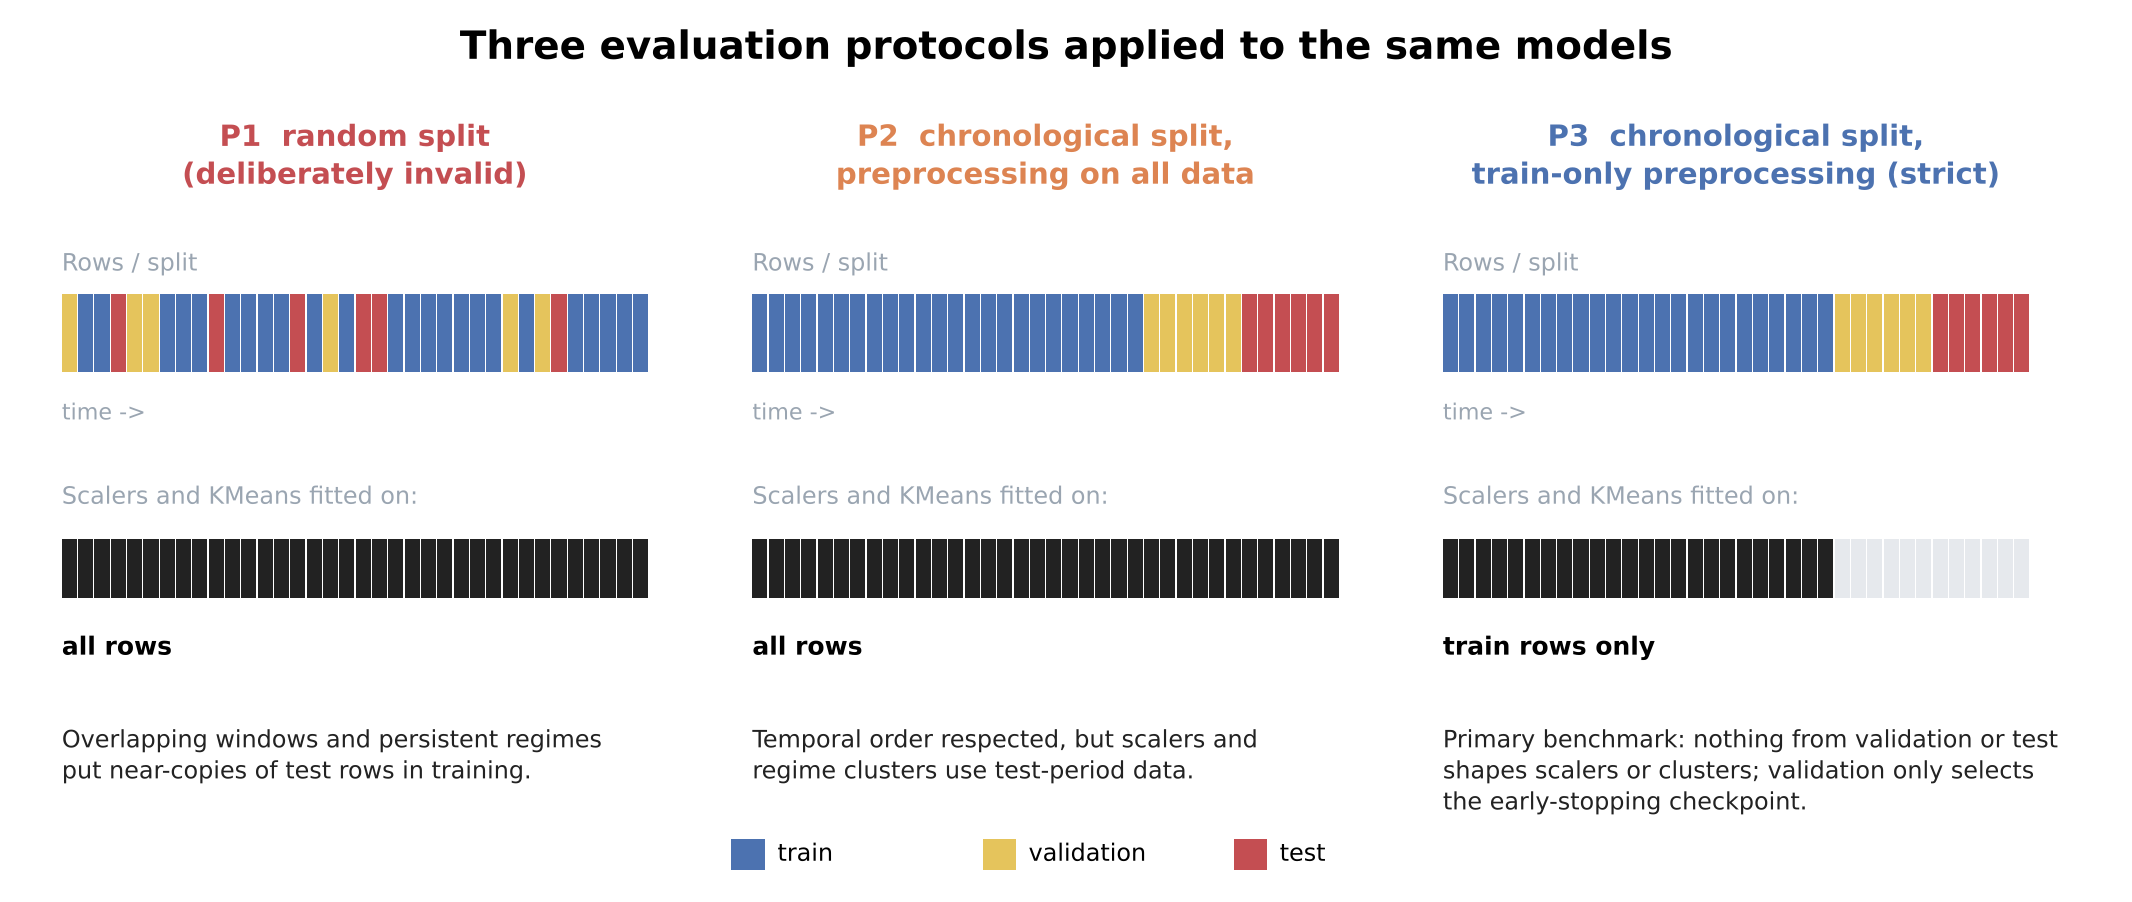
\includegraphics[width=\textwidth]{fig_protocol_design.png}
\caption{The three evaluation protocols. Dark squares in the lower strip mark the rows used to fit scalers and regime clusters.}\label{fig:protocols}
\end{figure}

\subsection{Statistical Inference}
\paragraph{Protocol gaps (RQ1).} For each model the gap is the difference between the mean test Macro-F1 under a looser protocol and under P3. A 95\% interval is obtained by bootstrapping the 10 per-seed scores of each protocol separately (1{,}000 resamples).
\paragraph{News value (RQ2).} For each group (all test rows, each regime, the stress window, and its complement), the seed-averaged predictions of each model are evaluated on test rows resampled with replacement (1{,}000 draws, the same resample for every model), and the difference in Macro-F1 between two models is computed on each resample. The 2.5th and 97.5th percentiles give the interval. These intervals describe test-set sampling uncertainty.
\paragraph{Stress window.} The stress window is 1 February to 30 April 2020 and contains 50 test rows; the regime groups contain 125 (Low-vol), 113 (Mid-vol) and 79 (High-vol) test rows.
\paragraph{Multiplicity.} About 24 pairwise comparisons are reported; an isolated interval that excludes zero is therefore treated as a hypothesis, not as a finding.

\subsection{Implementation}
All code is in Python with PyTorch, scikit-learn, pandas and the Hugging Face \texttt{transformers} library, and is available in the accompanying repository. FinBERT embedding was run on a GPU; models were trained on CPU in Google Colab. Training all models under all three protocols for ten seeds (270 runs) takes a few minutes on a CPU.
